\documentclass[12pt]{article}
\usepackage{import}
\usepackage{preamble}
\usepackage{environments}
% package for todo 
\setlength{\marginparwidth}{2cm}
\usepackage[colorinlistoftodos]{todonotes}
\setuptodonotes{size=\scriptsize,backgroundcolor=red!15!white} 

%\usepackage{showkeys} %show cites and refs

\title{Database Question: What has led to the dominance of Hamilton's quaternions, Heaviside's 3-dimensional vector algebra, and Grassmann's exterior algebra over Clifford algebras?}
\author{Colin Roberts}



\begin{document}

 \begin{titlingpage}
     \maketitle
     \vfill
     \begin{abstract}
        The topics in the title has interested me for quite some time. Each has found use for me in studying both pure mathematics and physics. My mathematical journey has taken me through each of the  of the topics listed and I have now settled on utilizing geometric algebras since they prove to simply contain all of the previously mentioned algebras in a more concrete manner. In fact, this is exactly why I have posed the proceeding question. One could argue that the rigorous notion of the Clifford algebras can be off putting, but if someone is interested in vector and linear algebra as a whole, a cursory understanding of Clifford algebras would allow one to build a strong foundation without needless rigor. For example, see the texts \cite{doran_lasenby_2013,chisolm_geometric_2012}. I believe there is a great deal of insight that Clifford algebras can provide a young mathematician over, say, Heaviside's approach, all without overbearing rigor or, conversely, lack of detail.

        As a final set of remarks, there seems to be two camps studying Clifford algebras. First, there are those who are deeply devoted and see it as a be-all end-all formalism that believe, unequivocally, that Clifford algebras are some type of holy grail of mathematics (see some of David Hestene's rants). The others are working predominantly in very pure fields who seem to use Clifford algebras in the most abstract and mind-bendingly rigorous way possible, thereby eclipsing adoption from mathematical youth who are driven away by overtly abject and complex technical jargon. One side question one could presume is, ``why is there such a dramatic divergence of scope for this topic?" Or, in the same vein, ``is there no middle ground for us to create a balanced viewpoint?" In writing this, I have discovered that these questions may be more fundamental than my original DBQ, but we carry on.
     \end{abstract}
 \end{titlingpage}


\section{Introduction}
The database question posed stems from a question I have been curious about since my introduction to Clifford algebras. Our key figures include William Rowan Hamilton, Hermann Grassmann, Josiah Willard Gibbs, Oliver Heaviside, and the less well-known William Kingdon Clifford. Of course, we may touch briefly on some other important mathematicians such as John Wallis and Felix Klein. Each member in this list had some role, be it direct or indirect, in the formulation of algebra that describes geometry. These algebras include the complex numbers, the quaternions, the Grassmann (or exterior) algebra, Gibbs/Heaviside vector algebra, and the enveloping Clifford algebras. One may take this foray and venture into the algebra of Pauli matrices or Dirac matrices as well.

I will attempt to give brief background in order to better immerse the reader into the topic. A mix of rigor will be used -- some elucidations will be more or less in depth than one may wish. Also, some prior knowledge will be assumed. At any rate, one will hopefully find curious relationships between these structures and, ideally, arrive at the same question posed earlier on their own. Throughout the introduction will be some brief historical remarks to set the stage for the primary sources and the subsequent commentary. For those familiar with the algebras stated above, you may feel free to move quickly or skip entirely the ensuing subsections. 

\subsection{Complex numbers}
The complex numbers find their origin quite long ago. There were references to square roots of negative numbers that may have appeared in Hero of Alaxandria's work in the first century AD. Studying polynomial equations led Gerolamo Cardano and Niccol\'o Tartaglia to consider complex numbers possibly as early as 1545. Ren\'e Descartes is given credit for providing the name ``imaginary". Later, we see complex numbers appear in Wallis' 1685 text \emph{A Treatise of Algebra} were formalized later into the complex plane by Caspar Wessel in 1799 in the text \emph{On the analytic representation of direction, an effort applied in particular to the determination of plane and spherical polygons}. 

To begin, one may first consider the complex number algebra $\C$ which adopts two key elements 1 and $i$. We note the identity 1 satisfies  $1^2=1$ whereas the imaginary unit $i$ satisfies $i^2=-1$. Taking $\R$ linear combinations of these elements by $x\cdot 1 + y \cdot i$ with $x,y \in \R$. We typically put $x+yi$ to reduce notational overhead and we reserve the binary operation $\cdot$ for later examples. Next, we see the addition and multiplication properties
\begin{align}
\label{eq:C_addition}
    x_1 + y_1 i + x_2 + y_2i  &= (x_1+x_2)+(y_1+y_2)i\\
\label{eq:C_multiplication}
    (x_1 + y_1 i)(x_2 + y_2i) &= (x_1x_2-y_1y_2)+(x_1y_2+x_2y_1)i,
\end{align}
where we have grouped terms to make the operations more clear. This algebra proves to be useful both algebraically and geometrically. The latter will prove to be of no surprise as we descend to more general structures.

In \cref{eq:C_addition}, we note that this addition mimics vector addition and Wessel argues that we can represent these numbers in a plane in order to realize this concretely. The role of $i$, however, is immense. For one, the fundamental theorem of algebra states that all polynomials over $\C$ (or any subring) have a full factorization in $\C$. Geometrically, $i$ acts as a rotor. Specifically, if I take a complex number $z$, $iz$ rotates the point $z$ by $\frac{\pi}{2}$ radians in the counter clockwise direction (see \cref{eq:C_multiplication}). Succinctly, algebra can lead to geometry. This theme is important.

Both the above realizations manifest themselves in other fields. For example, the fundamental theorem of algebra guarantees existence of Jordon forms for matrices as we can always find $n$-complex eigenvalues (possibly with repetition) for a linear operator on an $n$-dimensional vector space. Following from this, one finds that linear dynamical systems can be solved uniquely and the role of imaginary eigenvalues is to describe systems with rotations or oscillations. 

Lastly, and certainly not least, the complex algebra envelops many of the groups we typically see in introductory group theory courses. For example, symmetries of equilateral polygons are nicely encapsulated through multiplication of complex numbers. Perhaps this is most easily seen by the roots of unity $z^n=1$ for which we receive unique roots $z_1,\dots,z_n$ that form the vertices of an equilateral $n$-gon. Multiplication of these complex roots, for example, encodes the cyclic group of order $n$. Other symmetries utilizing complex numbers are prevalent in quantum mechanics, for example. Most generally, a rotation is given by an exponential $e^{i\theta}$.

\subsection{Quaternions}

The quaternions were independently discovered by Olinde Rodrigues in 1840 and later by Sir William Rowan Hamilton in 1843. As the story goes, Hamilton came to his realization on a walk passing over Brougham Bridge in Dublin where he scratched the famous equations
\begin{equation}
\label{eq:hamiltons}
i^2=j^2=k^2=ijk=-1
\end{equation}
in the stone. The quaternion algebra is the $\R$ algebra with the the basis elements 1, $i$, $j$, and $k$.

Much like the complex numbers describe rigid motions in the plane, the quaternions describe rigid motions in 3-dimensional space. Addition of purely imaginary quaternions, that is objects of the form $\alpha_1 i + \alpha_2 j + \alpha_3 k$, functions like 3-dimensional vector addition. Rotation in each plane can be captured via multiplication by certain elements. In fact, it comes down to the same exponential mapping for the complex numbers. Quaternions are used today in computer vision applications since they drastically simplify the computational overhead compared to matrices that are needed to compute rigid motions. 

It should be noted that the complex numbers arise as subalgebras of the quaternions. Indeed, any purely imaginary unit quaternion (so that $\alpha_1^2+\alpha_2^2+\alpha_3^2=1$) can be taken to act as the imaginary unit. Therefore we see that, for any axis we choose in space, there is a copy of $\C$ waiting there. Or, maybe more intuitively, for any plane in 3-dimensional space, we can induce a complex structure on the plane from a unit quaternion orthogonal to this plane. This is the isomorphism between the projective space and grassmannians 
\begin{equation}
\label{eq:isomorphisms}
\mathbb{RP}^3\cong \mathrm{Gr}(1,3)\cong \mathrm{Gr}(2,3).
\end{equation}
Grassmannians, named after Hermann Grassmann, leads us to our next icon.


\subsection{Grassmann algebra}

Hermann Grassmann developed his own take on a geometrically meaningful algebra which we now call the exterior algebra. His work beginning in 1832 formalized what we refer to as linear algebra. Later, in 1844, he published his \emph{theory of extension} which outlines the his algebra. Rather than just working in dimensions 2 or 3, Grassmann built this structure to encode some geometry of $n$-dimensional spaces. Given two vectors $u$ and $v$ in an $n$-dimensional vector space, he equipped another product $\wedge$ called the wedge (or exterior or outer) product satisfying
\begin{equation}
\label{eq:anticommutivity}
u \wedge v = - v \wedge u.
\end{equation}
The wedge product allows one to concatenate vectors into new objects of higher grade which seek to describe subspaces (or, really, linear combinations of subspaces). The elements have an orientation due to the anticommutivity property given in \cref{eq:anticommutivity}. These objects play a natural role in geometry as representations of $k$-dimensional volumes or $k$-vector fields. For example, given explicit $u$ and $v$, the wedge product can be used to output the area of an oriented parallelogram generated by $u$ and $v$. In the same vein, linear algebra operations such as the determinant are neatly captured in this algebra and the geometrical meaning becomes clear. For the case of the determinant, there is only a single grade $n$-vector and thus the product of $n$-vectors will describe the relative volume of an $n$-dimensional parallepiped that the vectors generate.

\subsection{Gibbs' and Heaviside's vector algebra}

Once again, two mathematicians independently discover the same idea. Starting in 1880, Gibbs followed the work of Grassmann to use the exterior algebra specifically for 3-dimensional space in order to produce the Maxwell equations. Heaviside was doing the same, and it is his version that we dominantly see today in a multivariate calculus course or course in electricity and magnetism. 

Both introduced the dot and cross products as the fundamental operations. The dot product provides the measure of lengths of vectors and can be used to determine angles between vectors. The curl, on the other hand, outputs information about areas generated by vectors as the wedge product of Grassmann did. However, the major difference is the cross product outputs another vector that is perpendicular to the plane generated by two independent vectors. But this is merely the same realization noted in the isomorphisms in \cref{eq:isomorphisms}.


\subsection{Clifford algebras}

At last, we arrive at our final key player, William Kingdon Clifford. Given the distinct advantage of coming last in our timeline of interest, Clifford was able to unify the above concepts into one single entity. We see the important quote from Henry John Stephen Smith that, ``Clifford was above all and before all a geometer." As such, though the work we examine is algebraic in nature, we expect the work to be rich in geometry.

In 1878, Clifford unifies the quaternions and Grassmann's algebra in his paper \emph{Applications of Grassmann's extensive algebra}. He equips a vector space not only with the product $\wedge$ but also includes an (psuedo)inner product $\cdot$ and incorporates this into the single geometric product. That is, the geometric product of vectors is
\begin{equation}
\label{eq:geometric_product}
uv = u\cdot v + u \wedge v.
\end{equation}
The geometric product places the $k$-vectors in the exterior algebra in the same footing as scalars and vectors. The inner product structure allows for a metric on the whole of the algebra and the geometric product allows for inverse operations. He referred to these algebras as geometric algebras.

The complex numbers can be seen as Clifford algebras or subalgebras in a handful of ways. For one, take $\R$ and define $e_1^2=-1$. Then, we have that $x+ye_1$ is a faithful representation of the complex number $x+iy$. Another way that is possibly more geometrically insightful is to consider $\R^2$ with $e_i^2=1$ and take the even subalgebra generated by $1$ and $e_1e_2$. Then $(e_1e_2)^2=-1$ and we can also note that $e_1e_2$ acts as a rotor for vectors in the plane. Indeed, we can refer to this as a spinor algebra. In fact, all elements in this algebra are generated by exponentials of bivectors, that is, any unitary even element can be written as $e^{\theta e_1 e_2}$. This is not surprising as for complex numbers we have the polar representation $re^{i\theta}$. 

The quaternions were a special case of a subalgebra of the larger geometric algebra on 3-dimensional space. The quaternions are ${{3}\choose{0}}+ {{3}\choose{2}}=4$-dimensional and the whole geometric algebra is of dimension $2^3$, i.e., the sum of all the binomial coefficients. Of course, the algebras exist for arbitrary dimensions. Clifford showed other examples of related algebras over different fields such as the complex field, the split-complex numbers, or dual numbers which could be used to form split-biquaternions or dual quaternions as well. When written as a geometric algebra, I will remark that if $e_1 e_2$ is a rotor for the $e_1 e_2$-plane, then it is clear that we have rotors for the other planes as well. These are the elements $i$, $j$, and $k$ of the quaternion algebra.

Notably, I shall mention that the choice of signature of the inner product produces more interesting algebras. For example, take a basis $e_1,\dots, e_4$ such that $e_i^2=1$ for $i=1,2,3$ and $e_4^2=-1$. This is often called the spacetime algebra which is used throughout relativity. From which, one can seek out to discover more about the Pauli and Dirac matrices.

\newpage

\section{The primary sources}

\subsection{A treatise of algebra, both historical and practical}

My first primary source is John Wallis' \emph{A treatise of algebra, both historical and practical} \cite{wallis_treatise_1685}.  This work provides a bit of a historical account of state of algebra at the time.

\begin{figure}[H]
    \centering
    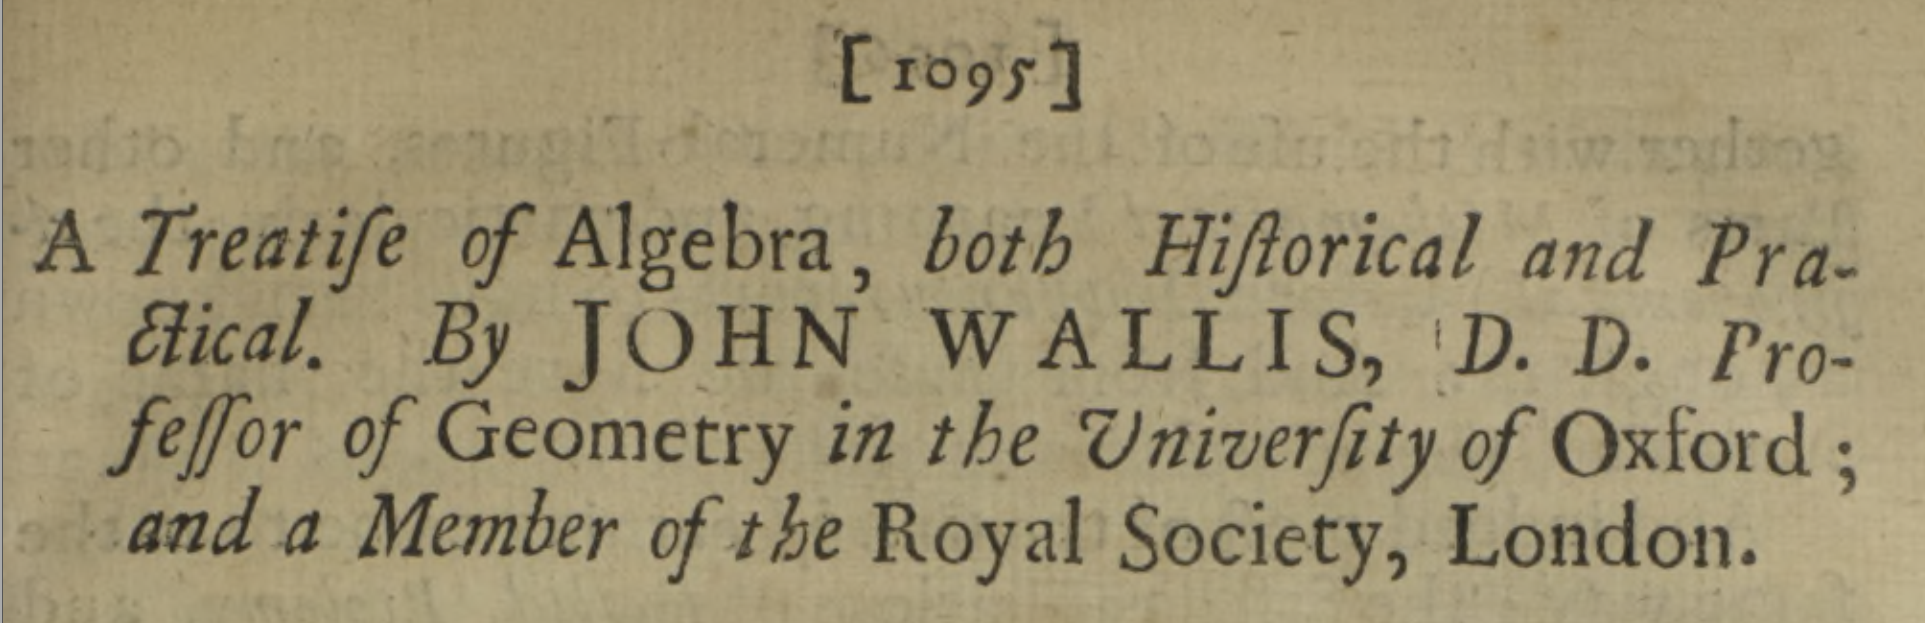
\includegraphics[width=.6\textwidth]{figures/wallis_title.png}
\end{figure}

For example, we can see Wallis mention the real and imaginary parts to roots. A great portion of this treatise is devoted to discussing the mathematicians who were working to solve and simplify polynomial equations.

\begin{figure}[H]
    \centering
    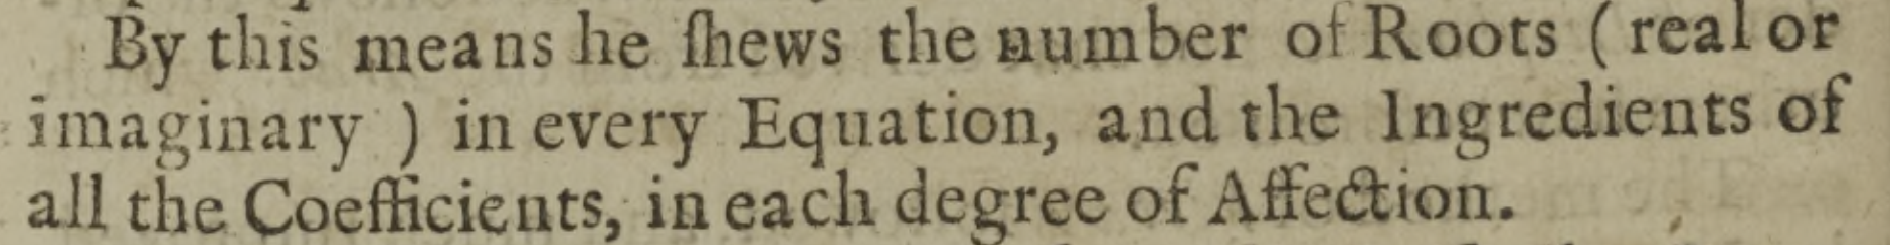
\includegraphics[width=.6\textwidth]{figures/wallis_imaginary.png}
\end{figure}

To get a full perspective of the development of Clifford algebras, it felt pertinent to start from the very beginning.

\newpage
\subsection{The linear extension theory - a new branch of mathematics}

The original document is in German and can be found via \cite{grassmann_lineale_1844} and the go-to english translation via this link \url{https://bookstore.ams.org/hmath-19}. 
\begin{figure}[H]
    \centering
    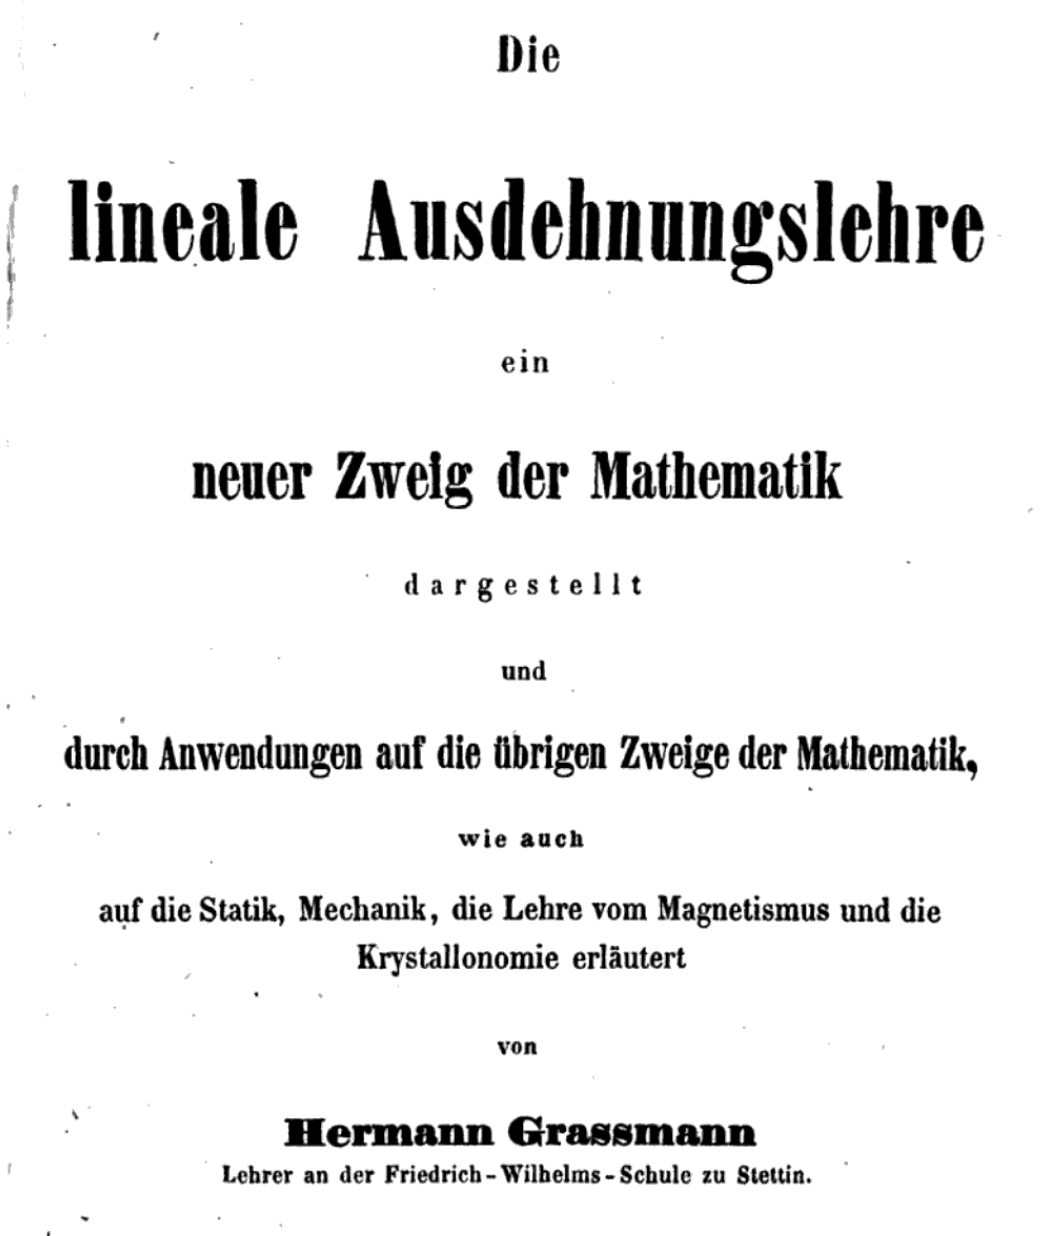
\includegraphics[width=.6\textwidth]{figures/grassmann_title.png}
\end{figure}

I am quite struck by the immense amount of groundwork that Grassmann lays out in his document. In essence, he describes our modern notions of linear algebra through his descriptions of elementary magnitudes. That is, elements that cannot be derived from one another -- or, in our more modern language, linearly independent vectors. Likewise, he notes that the complex numbers form an essential example for which he realizes are a foundation for understanding.

His claim to fame comes in the form of his antisymmetric product which he writes as $[ab]=-[ba]$ which we now write as $a\wedge b = - b \wedge a$. He uses this along with the inner product to build up geometrical interpretations of solutions to linear systems of equations. This general framework of linear algebra is essential to our story.

\newpage
\subsection{On quaternions, or on a new system of imaginaries in algebra}

Between 1844 and 1850 William Hamilton published \emph{On Quaternions; or on a New System of Imaginaries in Algebra}. Just a note, this is not an original scan of the multiple documents -- I have only been able to find a typed revision \cite{hamilton_quaternions_nodate}.  

Hamilton's work is beautiful. He aptly describes a completely new number system that extends the notion of imaginary numbers to a system with three imaginary components and a single real scalar. He begins by describing their products, length, and a polar representation which allows him to conclude that he has now described infinitely many different square roots of negative one. Thus, returning back to the original premise of complex numbers.

He is able to extract a large amount of geometry from this number system via algebraic equations by identifying the imaginary part of quaternions with points in space. In essence, it seems that he realizes there are two components to multiplication of quaternions -- the scalar product and some other type of product which we would think of as the cross or bivector product. It is clear that this is a heavy motivator for Clifford once his time comes.

\newpage
\subsection{A dynamical theory of the electromagnetic field}

Maxwell in 1865 publishes his text \emph{A dynamical theory of the electromagnetic field} \cite{maxwell_1865}. This was not his first paper on electromagnetism, but this is the source that seemingly describes the entirety of the theory as we know it today. The only difference is in notation. 

The belief at the time was that the electromagnetic field pervaded space as a type of fluid. This theme seems to be quite extensive in the history of physics -- fluids were usually used in place for some otherwise enigmatic entity. It's quite interesting to think this way about the electromagnetic field as there are great relationships between classical fluids and electromagnetism, for example, with plasmas.

This paper was a major turning point in physics. The electromagnetic theory is the first example of a truly fundamental theory of the universe, just ask Richard Feynman. If you are asked to explain why electromagnetism behaves the way it does, there is no other way to answer this other than to essentially just say that ``it is so."

\newpage

\subsection{Applications of Grassmann's extensive algebra}

Finally, we arrive at some work by Clifford himself. In 1878, William Clifford published \emph{Applications of Grassmann's Extensive Algebra} \cite{clifford_applications_1878}. We see that Clifford merely takes the axiom that we have orthogonal magnitudes such that $e_i e_j = -e_j e_i$ when $i\neq j$. This is the fundamental assumption for a geometric algebra. He realizes that there is more to the multiplication for quaternions than the two products of Grassmann in that the quaternion multiplication encapsulates ``turning and stretching". He realizes the quaternions as ``rectangular versors" (i.e., what we realize as $e_i e_j$ for $i\neq j$ in dimension 3). Purely by geometry, he reasons that these elements, when squared, should reverse a vector (that is, for example, $(e_1 e_2)^2=-1$). Perhaps, this makes Henry Smith's quote ``Clifford was above all and before a geometer," more reasonable!

Clifford reunites the quaternions with Grassmann's extensive algebra and, quite clearly, also realizes the complex field as a special case in dimension 2 as well. He then describes, in general, the geometric algebra for $n$-dimensional space.

\newpage
\subsection{On the space-theory of matter}

In 1882, Clifford publishes a text including many short papers \cite{clifford_1882}. One of which is titled \emph{On the space-theory of matter} which contains Clifford's comments on whether we live in a curved universe. I found it quite intriguing that his geometry led him down this same path prior to Einstein. Also, you can find his general comments on Riemann surfaces as well.

Clifford was very interested in non-Euclidean geometry that was being developed at this time and thought that it was an ideal setting for physics. So, he followed much of the work of Gauss and Riemann.


\newpage
\subsection{Electromagnetic theory}

Later on, in 1894, Oliver Heaviside published his book \emph{Electromagnetic theory} for which I cite a single chapter \cite{heaviside_2011_vec}. This text may indeed be the crux of the argument posed by my DBQ.

Here, we see Heaviside bring forth our modern notion of vector algebra and calculus. Yet, it is some tailormade approach that is specifically formulated solely for the describing the mechanisms of electromagnetism. He uses the same notation as Hamilton to represent basis vectors in $\R^3$, that is, $i$, $j$, and $k$. Yet, he determines the squares $i^2=j^2=k^2=1$, which we should recognize as the scalar product and he indeed refers to this as such. In that same sense, he finds it clear to say $ij=jk=ki=0$. This is different than both Hamilton, Grassmann, or Clifford would have argued!

It is rather remarkable; the notation and formalism used by Heaviside is exactly how we teach students today. He describes the how any vector can be written as a sum of $i$, $j$, and $k$ and builds up the geometries of parallelograms and parallelepipeds using scalar products. He also describes the vector product (the cross product) which inputs two vectors and outputs a vector perpendicular to both. 

\newpage
\subsection{The quantum theory of the electron}

Finally, I chose the source of Dirac on \emph{the quantum theory of the electron} \cite{dirac_quantum_1928}. This inclusion may seem out of place, but I contest that it may have some to do with my DBQ.

\begin{figure}[H]
    \centering
    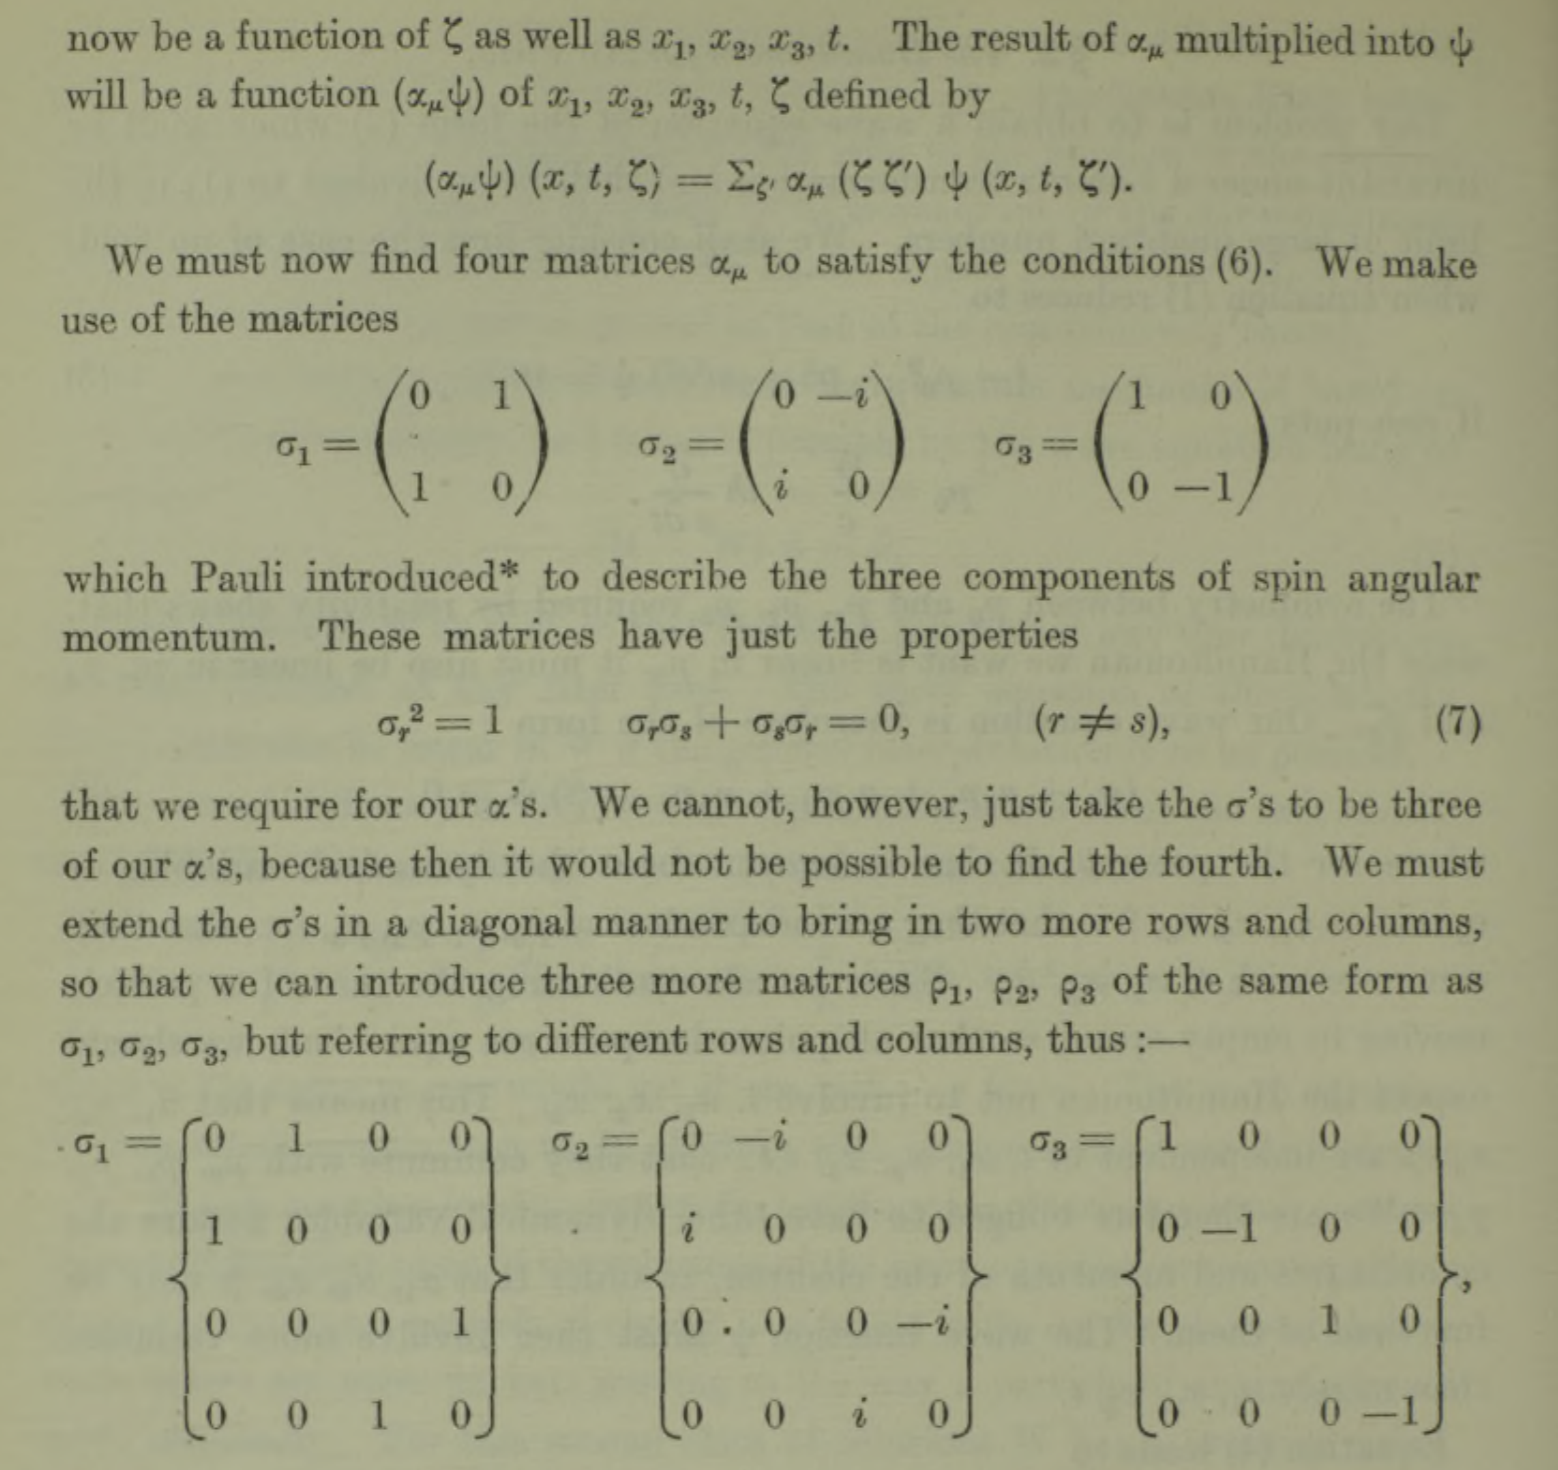
\includegraphics[width=.6\textwidth]{figures/dirac_matrices.png}
\end{figure}

It is abundantly clear that Dirac is of dire importance to modern physics. This paper of his is paramount. But, the catching point is his matrices $\sigma_i$. Herein lies an issue. Dirac needed no help to realize that he could generate square roots to a relativistic wave equation for which he has two new equations which allowed him to find two (spinor) solutions. These $\sigma_i$ are in fact, elements of the spacetime algebra -- he just had no need of using this formalism and instead used matrices as his convention. 


\newpage
\section{Commentary}

Let us start from the beginning and crawl forward through these documents cohesively. 

First, take note of just how enriching the complex algebra is. Not only do we receive the fundamental theorem of algebra (which was realized quite long ago), but we develop a since of planar geometry through algebra. Grassmann is able to deduce that the elements 1 and $i$ are fundamental, and cannot be decomposed further. As such, all points are really combinations of these two entities. Then, we also know how to multiply and add complex numbers which shows us their scaling and rotation properties.

Grassmann carried on to develop much more. The foundation of linear algebra as we know it today was given to us by him. Not only that, but his geometrical insight allows us to develop a formal version of calculus for which we can handle oriented $k$-dimensional objects. His description of the geometry given to us by linear algebra paved way for modern manifold theory since, locally, the whole theory reduces to linear and exterior (or, extensive) algebra.

Hamilton sees this all in another way. Based on my own interpretation, I believe he was searching for a new system of numbers that were more general than the complex numbers. This is reasonable. The complex numbers encode planar geometry and, since we live in 3-dimensional space, there should be numbers that encode this geometry as well. He manages to discover the famous set of quaternions with their relationship mimicking the complex numbers. Three additional units whose squares are negative one. His deep dive showed us all that these quaternions do indeed model the stretching, reflecting, and rotating of space that we are familiar with.

Next comes Clifford who shows the world that what Grassmann and Hamilton are describing are completely compatible and they are part of a more general notion of a geometric algebra. For which, Clifford describes a product that unites the scalar product and the exterior product. The key insight is that he realizes, for example, that planar elements on Grassmann's algebra are the same as the elements that rotate space in Hamilton's algebra and hence he calls them rotors (what we may now call now, due to Pauli and Dirac, spinors). In fact, he shows you can build more general structures via products of vectors whose actions should be intuitive.

Products of vectors represent geometrical structures. For example, the product of sums of vectors in space yields scalar elements, vector elements, planar elements, and volume elements. He discusses the impact of the dimension of the underlying space and whether they are flat, hyperbolic, or parabolic, and how that effects these algebras. This, in or modern version of Clifford algebras, is the signature of the quadratic form. 

Clifford was also working on a way of describing physics through the geometry of space. The amazing fact here is that Clifford algebras are deeply tied to the spacetime of Einstein. For example, the inner product defined on Minkowski space is what Clifford would think of as hyperbolic. General relativity can be formulated using Clifford algebras and I find myself curious as to how far along Clifford got in his short life.

Maxwell published his papers on the electromagnetic theory before Clifford published the papers I reference. It seems that his was also motivation for Clifford to try and describe this physics in particular through his geometric algebra. In fact, the geometric algebra formalism aptly describes electromagnetism and distinguishes between the characteristics of the electric vector field and magnetic bivector field. Clifford even mentions that Maxwell discusses force and flow which he realizes as linear functions and binary products.

Yet, we find ourselves at the date of Heaviside. His work was heavily based on Grassmann's extensive algebra but has insight from Hamilton as well (as made clear by notation). He defines the scalar product analogously and he defines a cross product in that he simply chooses to pick a vector perpendicular to the plane generated by $a \wedge b$. But, in Clifford's terms, he really chooses an element $(a\wedge b)^\perp$, where $\perp$ is multiplication by the top degree element (pseudoscalar). This is a notion of duality. At this point, he realizes
\[
i\times j = k,\quad j \times k = i, \quad k\times i = j,
\]
which mimics Hamilton's quaternion multiplication. In fact, this is a realization of the duality of the wedge in that
\[
(a \wedge b)^\perp = a^\perp \boldsymbol{\times} b^\perp,
\]
where $\boldsymbol{\times}$ is the bivector commutator product. So, it seems that Heaviside in his attempt to succinctly describe 3-dimensional phenomenon overlooks this relationship. That, instead of using the single product of Clifford, breaks the product apart into those of Grassmann and Hamilton. He finds only a use in vector quantities and ignores elements of differing grade. But, Heaviside's treatment of electromagnetism was very usable and electromagnetism was the forefront of the mathematical and physical world at the time. Thus, this theory was launched into the lead and we kept only bits and pieces of the necessary insight from Hamilton and Grassmann but far less so of Clifford.

Clifford had built his theory off of giants such as Hamilton and Grassmann. Yet, his implementation seemed mostly formal. Though it unified a landscape of mathematics, it was not a necessity like Grassmann's or Hamilton's work. Those two pieces were very pioneering and the need to do physics at the time reigned over the importance of a general schema in math.So, Clifford was to remain as a historical sidenote in comparison. But, it is clear to me that Clifford was an intelligent man that was quite far ahead of his time. If someone can predict the work of Einstein before Einstein, they are certainly bright. Yet, due to the fact that his work was not required to solve problems and was really only an encapsulating framework, authors like Dirac managed to sidestep the notion of a geometric (or Clifford) algebra in lieu of matrices. I should say that there are many bright icons of physics and math out there that did reach a level of fame and this does not mean Clifford should be treated as some surreptitious spectacle who we must pay special homage to.

As mentioned just previously, Dirac enters the equation with his treatment of the electron. This all takes place after Einstein's general theory of relativity which would have delighted Clifford. Electromagnetism and gravity were in attempt to be united together in a single force by Einstein and others. Einstein, however, avoided the quantum world where Dirac seemed to live in. So, Dirac manages to further our understanding of the electromagnetic theory where, again, we see Clifford's geometric algebras arise. Yet, there was again no need to refer to this -- matrices served their purpose just as Heaviside's formalism did. In fact, we even see that the natural derivative operator in Clifford analysis is often referred to as the Dirac operator.

Yet, there is a connection between the relativity of Einstein and the theory of Dirac. Their coupling lies in the spacetime algebra which is used for both theories. I am not suggesting some theory of everything, but what I do want to suggest is that the global perspective of Clifford should really not be ignored. Circumstance led to Clifford's ideas to be just the shadows of the giants we have all heard. 

I do not think I have managed to answer the question posed as there is just far more to unpack that may lead to a more fulfilling story. But, I can say that it was enriching to see the unfolding of our modern notions of linear algebra, geometry, electromagnetism, and relativity through a historical lens. I'm interested to see if I can find more over time. 

As for my other two questions posed at the end of my abstract, I cannot tell you for certain, but I will make some comments. It is likely that there is no clear reason other than the individuals who have involved themselves in this story line have their own personalities and these personalities manifest themselves through their writings. Once this has begun, others identify with their chosen groups which leads to the divergence I mention.

Is there a middle ground for us to create a balanced viewpoint? The answer to me is clear -- yes. Why not? There is absolutely no issue in exploring mathematics that is not frontpage news. In fact, I'd argue there are many open questions in areas like this that, through research, could lead to connections yet unknown. There has been a resurgence of Clifford's work since the 1980's and modern texts published as of 2013, and I am curious to see how this plays out during my mathematical career.



\bibliographystyle{siam}
\bibliography{dbq}





\end{document}
